\begin{figure}[t]
	\begin{minipage}[b]{0.49\linewidth}
		\centering
		\centerline{ 
\includegraphics[width=\textwidth]{disp} }
		\centerline{(а) Оцененная карта диспаратности}\medskip
	\end{minipage}
	\hfill
	\begin{minipage}[b]{0.49\linewidth}
		\centering
		\centerline{
\includegraphics[width=\textwidth]{wmf} }
		\centerline{(б) Улучшенная карта диспаратности}\medskip
	\end{minipage}
	\begin{minipage}[b]{1\linewidth}
		\centering
		\centerline{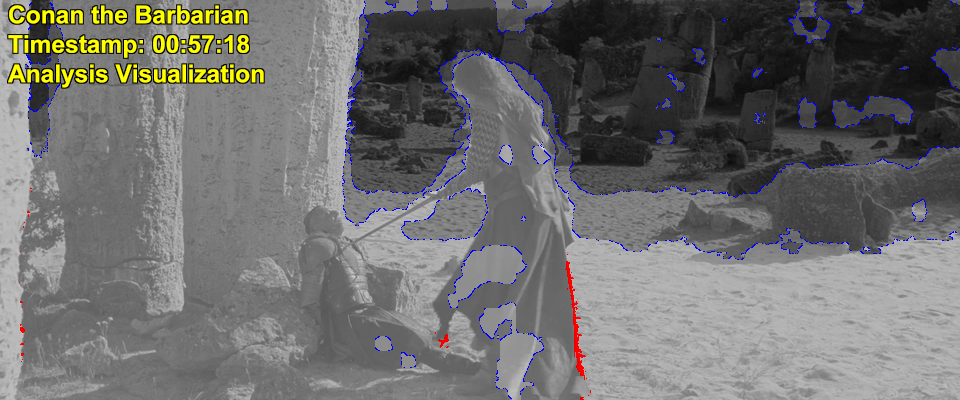
\includegraphics[width=\textwidth]{visualization} }
		\centerline{(в) Визуализация конечного результата}
	\end{minipage}
    \caption{Примеры карт диспаратности перед~(а) и после~(б) фильтрации 
    	взвешенной медианы. Итоговая визуализация~(в), которая предлагается
    	в качестве одного из выходов алгоритма, содержит карту диспаратности поверх 
    	исходного кадра. Синий цвет отмечает границы диспаратности, а красный---
    	несоответствия между границами карт  амплитуды движения и диспаратности.}
	\label{fig:disp}
\end{figure}
